% figure: 青大825-2019-第3题结构图.png
% 用途：2019 青岛大学825 第3题 —— 系统结构图（原卷为扫描图，本图按答案解析的
%       节点关系重构：e=R-G4·G1e，C=G1e+G2(e-G3C)，故 C/R=(G1+G2)/[(1+G1G4)(1+G2G3)]）
% 构建：..\build.ps1 -File .\exam-2019-t3.tex
\documentclass[border=10pt]{standalone}
\usepackage{fontspec}
\setmainfont{Cambria}
\usepackage{unicode-math}
\setmathfont{Cambria Math}
\usepackage{tikz}
\usetikzlibrary{positioning, arrows.meta, calc}
\usepackage{ctex}

\definecolor{figink}{HTML}{1E2228}
\definecolor{figsub}{HTML}{606874}
\definecolor{figfill}{HTML}{E8EFF8}

\begin{document}
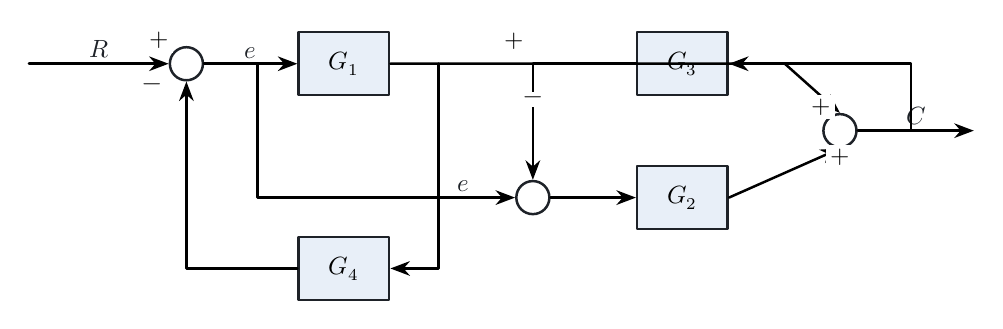
\begin{tikzpicture}[
  x=1cm, y=1cm,
  line width=0.9pt, line cap=round, line join=round,
  >=Stealth,
  blk/.style  = {draw=figink, line width=0.9pt, fill=figfill,
                 minimum width=1.15cm, minimum height=0.8cm, inner sep=2pt,
                 anchor=center, font=\small},
  sum/.style  = {draw=figink, line width=0.9pt, circle, inner sep=0pt,
                 minimum size=0.42cm, anchor=center},
  sig/.style  = {font=\small, color=figink, fill=white, inner sep=1.5pt},
  lbl/.style  = {font=\small, inner sep=1.5pt, fill=white}
]

% 节点：上支路 y=0，下支路 y=-1.7
\node[sum] (s)   at (0,0)     {};
\node[blk] (g1)  at (2.0,0)   {$G_1$};
\node[sum] (s2)  at (4.4,-1.7){};
\node[blk] (g2)  at (6.3,-1.7){$G_2$};
\node[sum] (sy)  at (8.3,-0.85){};
% 反馈块
\node[blk] (g4)  at (2.0,-2.6) {$G_4$};
\node[blk] (g3)  at (6.3,0)    {$G_3$};

% R -> e
\draw[->] (-2.0,0) -- node[sig, above] {$R$} (s.west);
% e -> G1 -> 上支路 -> 输出加法器
\draw[->] (s.east) -- node[sig, above] {$e$} (g1.west);
\draw[->] (g1.east) -- (7.6,0) -- (sy.north);
% e -> G2 -> 输出加法器
\draw[->] (s.east) -- (0.9,0) -- (0.9,-1.7) -- node[sig, above, pos=0.8] {$e$} (s2.west);
\draw[->] (s2.east) -- (g2.west);
\draw[->] (g2.east) -- (sy.south);
% 输出
\draw[->] (sy.east) -- node[sig, above] {$C$} (10.0,-0.85);

% 上回路：G1 输出 --G4--> 链首加法器
\draw[->] (3.2,0) -- (3.2,-2.6) -- (g4.east);
\draw[->] (g4.west) -- (0,-2.6) -- (s.south);
% 下回路：C --G3--> G2 前加法器
\draw[->] (9.2,-0.85) -- (9.2,0) -- (g3.east);
\draw[->] (g3.west) -- (4.4,0) -- (s2.north);

% 符号
\node[lbl] at (-0.34,0.30) {$+$};
\node[lbl] at (-0.44,-0.30) {$-$};
\node[lbl] at (4.16,0.28)  {$+$};
\node[lbl] at (4.4,-0.46)  {$-$};
\node[lbl] at (8.06,-0.55) {$+$};
\node[lbl] at (8.3,-1.19)  {$+$};

\end{tikzpicture}
\end{document}
